\documentclass{article}

% if you need to pass options to natbib, use, e.g.:
%     \PassOptionsToPackage{numbers, compress}{natbib}
% before loading neurips_2021

% ready for submission
\usepackage[final]{neurips_2021}

% to compile a preprint version, e.g., for submission to arXiv, add add the
% [preprint] option:
%     \usepackage[preprint]{neurips_2021}

% to compile a camera-ready version, add the [final] option, e.g.:
%     \usepackage[final]{neurips_2021}

% to avoid loading the natbib package, add option nonatbib:
%    \usepackage[nonatbib]{neurips_2021}

\usepackage[utf8]{inputenc} % allow utf-8 input
\usepackage[T1]{fontenc}    % use 8-bit T1 fonts
\usepackage{hyperref}       % hyperlinks
\usepackage{url}            % simple URL typesetting
\usepackage{booktabs}       % professional-quality tables
\usepackage{amsfonts}       % blackboard math symbols
\usepackage{nicefrac}       % compact symbols for 1/2, etc.
\usepackage{microtype}      % microtypography
\usepackage{xcolor}         % colors

\usepackage{graphicx}
\usepackage{caption}
\usepackage{subcaption}
\usepackage{float}

\usepackage{amsmath,amscd,amssymb,amsthm}
\usepackage{cases}
\usepackage{thmtools}
\usepackage{thm-restate}
\usepackage{mdframed,url,multirow,listings,textcomp,ifthen}   
\usepackage{tikz,mathtools,color}
\usepackage{parskip}

\newtheorem{theorem}{Theorem}[section]
\newtheorem{corollary}{Corollary}[theorem]
\newtheorem{lemma}[theorem]{Lemma}

\newcommand{\R}{\mathbb{R}}
\newcommand{\E}{\mathop{\mathbb{E}}}
\newcommand{\argmin}{\mathop{\text{argmin}}}
\newcommand{\argmax}{\mathop{\text{argmax}}}
\newcommand{\Regret}{\text{Regret}}
\newcommand{\Wealth}{\text{Wealth}}
\newcommand{\diag}{\text{diag}}
\renewcommand{\L}{\mathcal{L}}

\newcommand{\bx}{\mathbf{x}}
\newcommand{\bxt}{\mathbf{\tilde x}}
\newcommand{\by}{\mathbf{y}}
\newcommand{\bw}{\mathbf{w}}
\newcommand{\bz}{\mathbf{z}}
\newcommand{\bv}{\mathbf{v}}
\newcommand{\bg}{\mathbf{g}}
\newcommand{\bu}{\mathbf{u}}
\newcommand{\bq}{\mathbf{q}}
\newcommand{\FTRL}{\text{FTRL}}
\newcommand{\OSD}{\text{OSD}}
\newcommand{\op}{\text{op}}
\renewcommand{\H}{\mathbf{H}}
\newcommand{\todo}[1]{\textcolor{red}{#1}}

\title{A Scale-Free MADGRAD Regret Bound}

% The \author macro works with any number of authors. There are two commands
% used to separate the names and addresses of multiple authors: \And and \AND.
%
% Using \And between authors leaves it to LaTeX to determine where to break the
% lines. Using \AND forces a line break at that point. So, if LaTeX puts 3 of 4
% authors names on the first line, and the last on the second line, try using
% \AND instead of \And before the third author name.

\author{
  Shashank Manjunath \\
  Boston University \\
  \texttt{manjuns@bu.edu} \\
}

\begin{document}

\maketitle

\todo{\section{Introduction}}

This project is concerned with dual averaging algorithms applied to deep learning. So far, we have tested two dual
averaging algorithms, Modernized Dual Averaging (MDA) (\cite{jelassi_dual_2020}) and MADGRAD
(\cite{defazio_adaptivity_nodate}), which use Follow the Regularized Leader (FTRL) style algorithms in order to optimize
deep learning algorithms. For this project, we have focused on both implementing these algorithms in PyTorch
(\cite{paszke_pytorch_2019}) and testing them out on the CIFAR10 dataset (\cite{krizhevsky_learning_nodate}). We then
prove an alternate, scale-free regret bound for the MADGRAD algorithm.

\todo{\section{Algorithm Details}}

\todo{\section{Algorithm Implementation}}

So far, we have successfully replicated results on the CIFAR10 dataset for the MDA, MADGRAD, Adam, and Stochastic
Gradient Descent with Momentum (SGD+M) algorithms. We show our test accuracy and test loss results in the plot below.

\begin{figure}[H]
  \centering
  \begin{subfigure}{.5\textwidth}
    \centering
    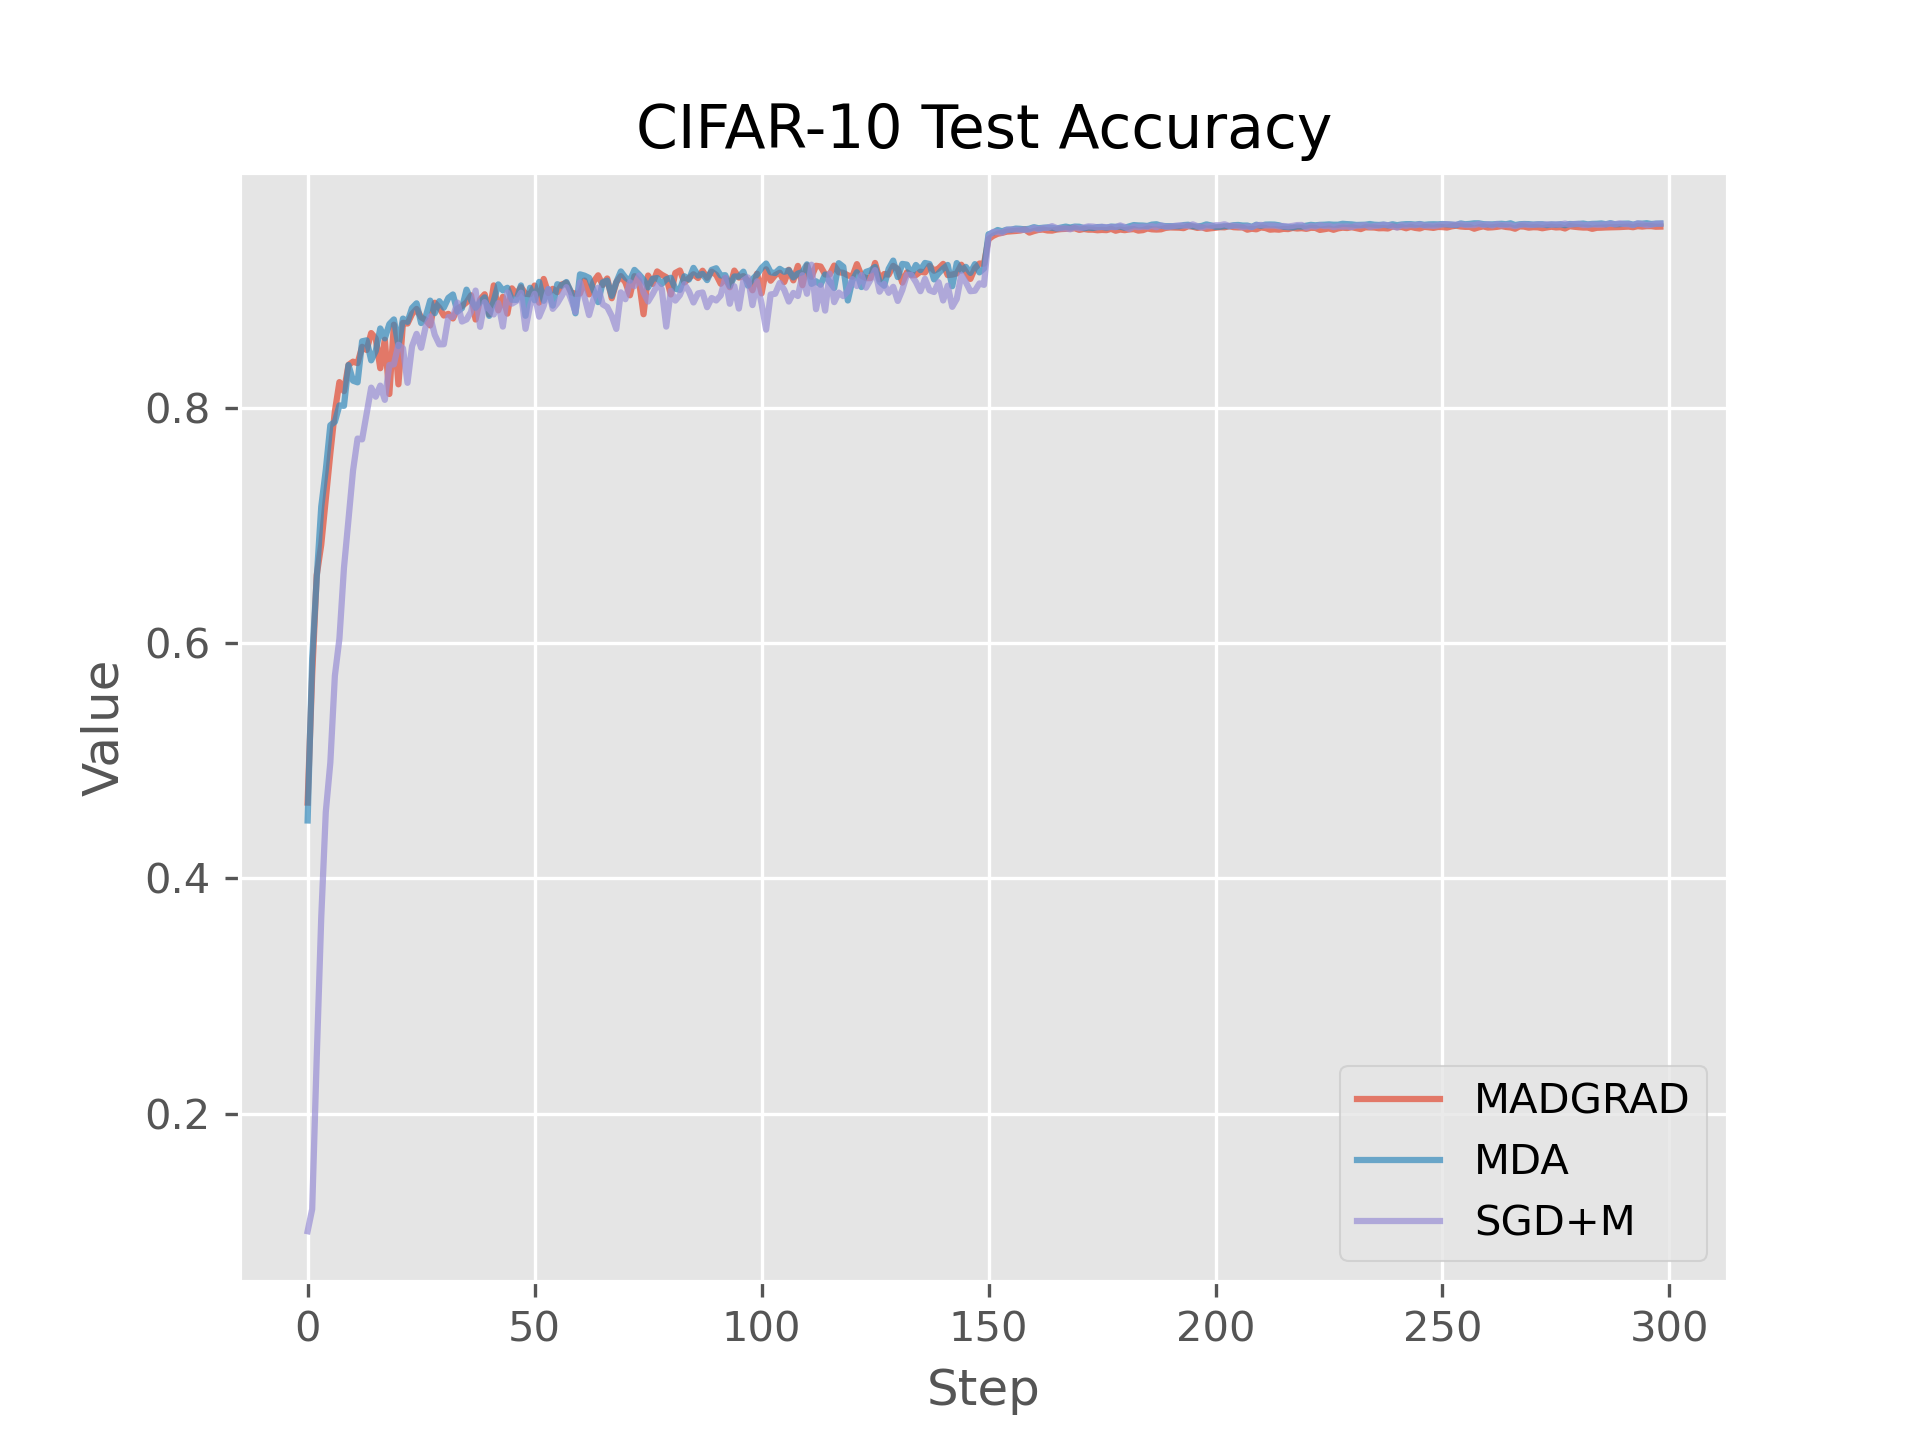
\includegraphics[width=\linewidth]{../ftrl_dl_data/CIFAR-10_test_acc.png}
    \caption{Test Accuracy of Optimizers on CIFAR-10}
    \label{fig:sub1}
  \end{subfigure}%
  \begin{subfigure}{.5\textwidth}
    \centering
    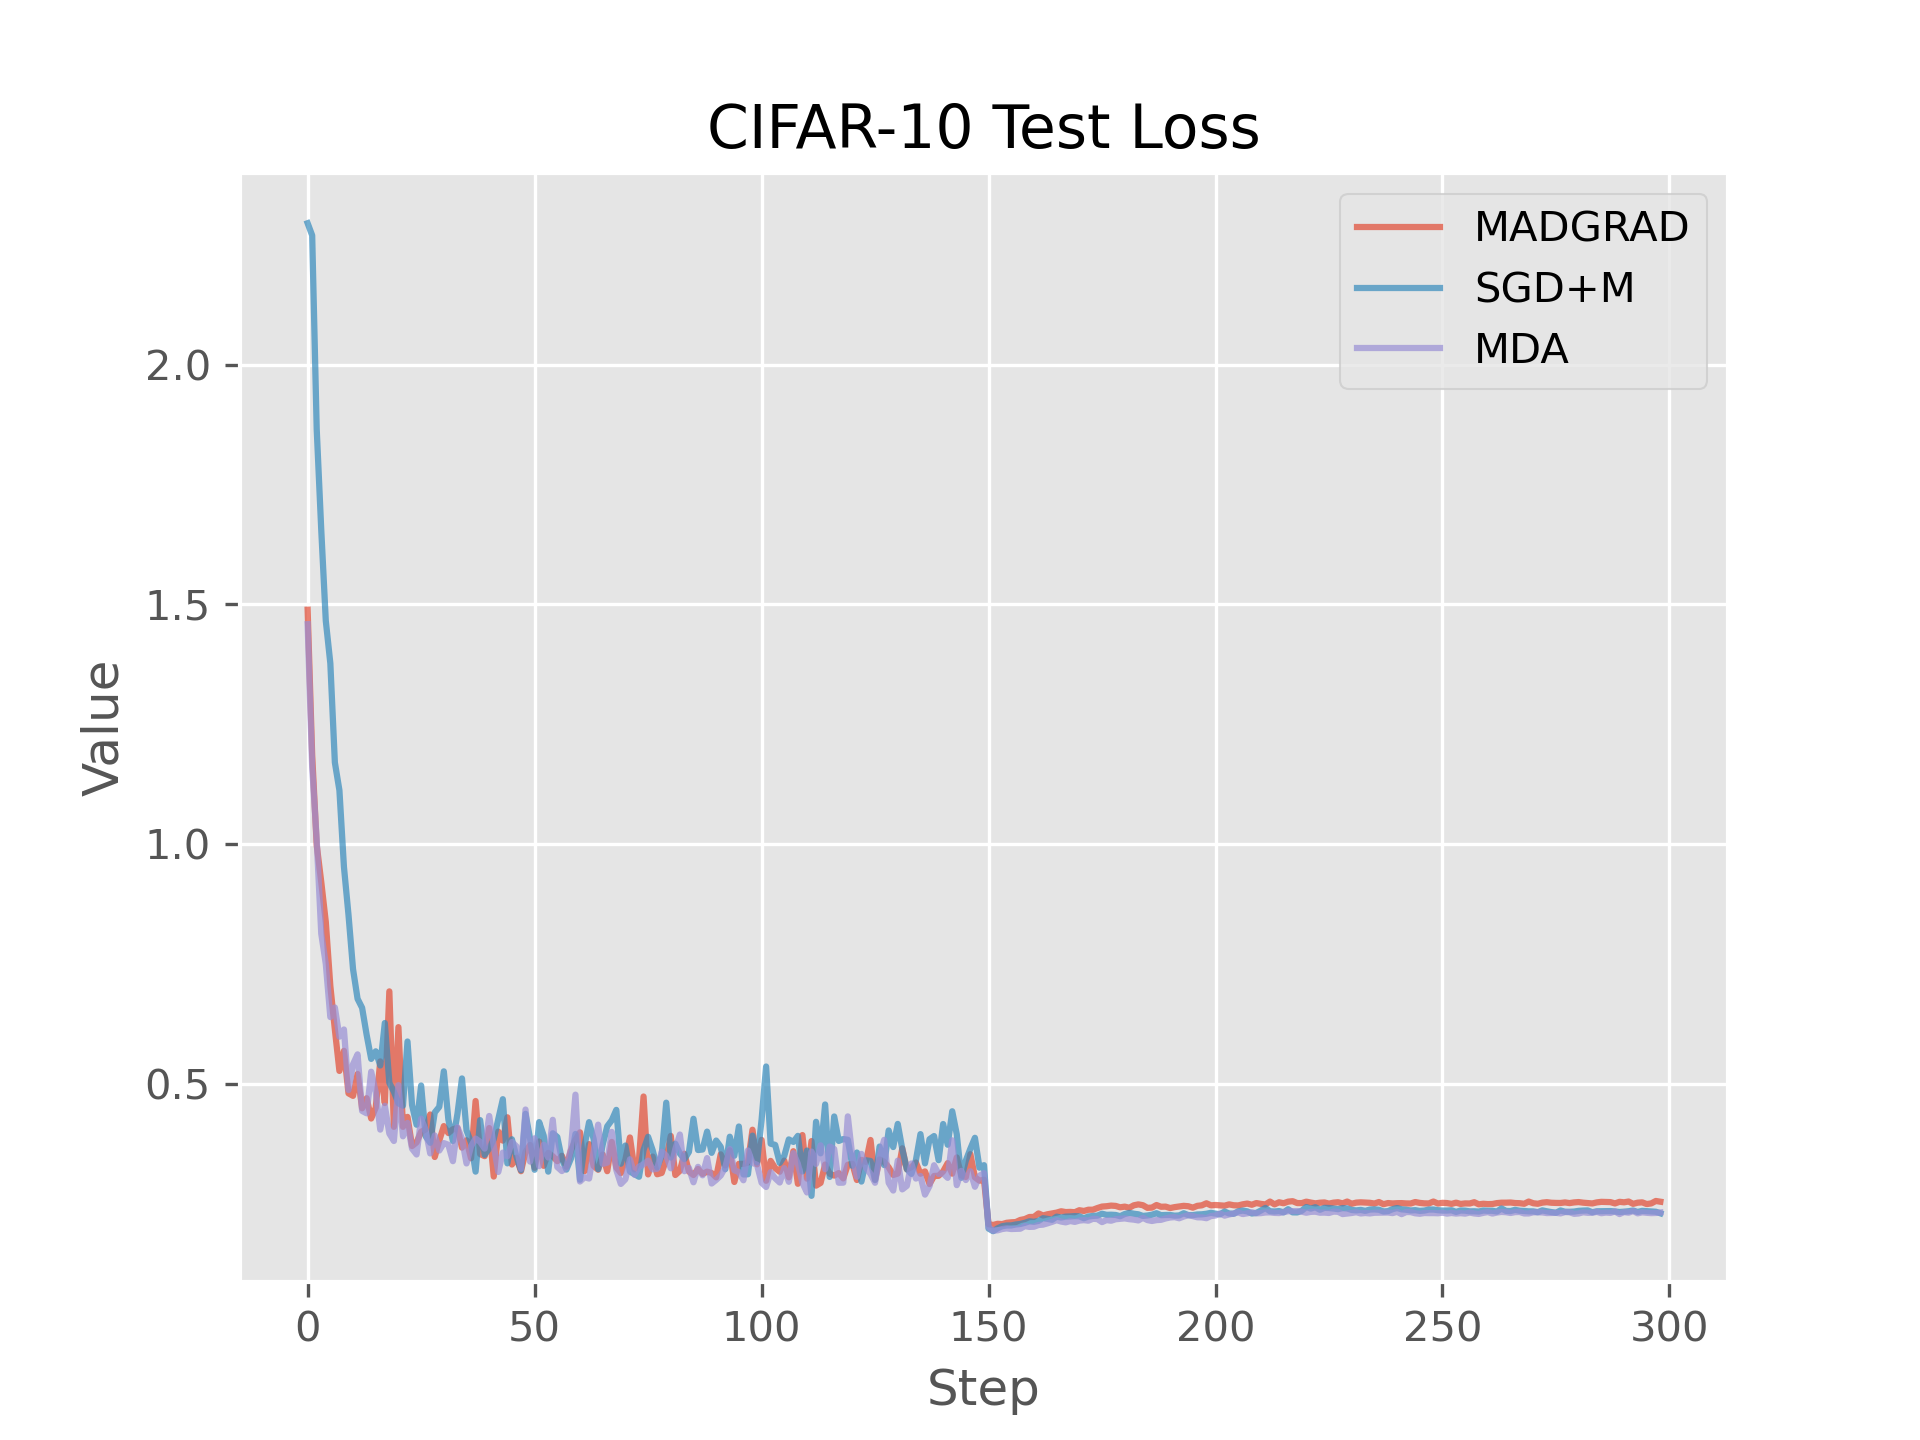
\includegraphics[width=\linewidth]{../ftrl_dl_data/CIFAR-10_test_loss.png}
    \caption{Test Loss of Optimizers on CIFAR-10}
    \label{fig:sub2}
  \end{subfigure}
  \caption{Comparison of optimizer performance on CIFAR-10 dataset}
  \label{fig:test}
\end{figure}

Our experiment setup and optimizer implementations for MDA and MADGRAD can be found at
\url{https://github.com/shashankmanjunath/ftrl_deep_learning}.

\section{Theory}

While studying the convergence proof for the MADGRAD algorithm, we identified a potential improvement on the existing
theory. 

\todo{make above line sound more professional}

When proving the convergence bound for MADGRAD, the authors require an alternative definition of
MADGRAD than the one presented in the paper and implemented. In the original MADGRAD algorithm presented in the paper,
the $z_{k+1}$ is given by:

\[
  z_{k+1} = x_0 - \frac{1}{\sqrt[3]{v_{k+1}} + \epsilon} \circ s_{k+1}
\]

where $\circ$ indicates the Hadamard product. $\epsilon$ is included for numerical stability in the early iterations of
the algorithm, as the $v_{k+1}$ parameter can be 0. However, in the convergence proof, the $z_{k+1}$ parameter is given
by:

\[
  z_{k+1} = x_0 - \frac{1}{\sqrt[3]{\lambda_{k+1}G^2 + v_{k+1}}} \circ s_{k+1}
\]

Note the extra $\lambda_{k+1}G^2$ in the denominator, which is used to create the following upper bound leveraged in the
overall convergence proof:

\[
  \sum\limits_{t=0}^k \frac{\lambda_t^2 g_t^2}{\sqrt[3]{\lambda_t G^2 + \sum\limits_{i=0}^{t-1} \lambda_i g_i^2}} \leq
  \frac{3}{2} \lambda_k \left(\sum\limits_{i=1}^k \lambda_i g_i^2\right)^{\frac{2}{3}}
\]

This extra $\lambda_t G^2$ prevents the algorithm from being \emph{scale-free}, or an algorithm that is invariant to the
scaling of losses by a constant factor. Therefore, we aim to construct a convergence proof which maintains the
scale-free nature of the algorithm.

\subsection{Proof of Scale-Free Regret Bound for MADGRAD}

Consider the MADGRAD algorithm. This algorithm implements the regularizer: 

\[
  \psi_t(\bx) = \frac{1}{2} \|\bx - \bx_0 \|_{A_t}
\]

where $A_t = \diag(\alpha_t)$, and $\alpha_t = \sqrt[3]{\sum\limits_{i=1}^{t-1}\lambda_i g_i^2}$. Note that
$\psi_t(\bx)$ is strongly-convex with respect to the norm $\| \cdot \|_{A_t}$. Let us denote the Bregman divergence by
$B$ and let $\theta_t = \sum\limits_{i=1}^t g_i$, where $g_t$ is the subgradient of the algorithm at round $t$. Let us
first define some useful lemmas.

\begin{lemma}[Lemma 1 in \cite{orabona_generalized_2014}]
  Let $\{\psi_t\}_{t=1}^\infty$ be a sequence of functions defined on a common convex domain $S \subseteq \R^n$ and
  such that each $\psi_t$ is $\mu_t$-strongly convex with respect to the norm $\|\cdot\|_t$. Let $\|\cdot\|_{t, \star}$ be
  the dual norm of $\| \cdot \|_t$, for $t = 1, 2, \cdots, T$. Then, for any $\bu \in S$,

  \[
    \Regret _T (\bu) \leq \sum\limits_{t=1}^T \langle g_t, \bu - \bx_t \rangle \leq \psi_{T}(\bu) + \psi_{1}^\star (0) +
    \sum\limits_{t=1}^T B_{\psi_{t}^\star}(-\theta_t, -\theta_{t-1}) - \psi_{t}^\star (-\theta_t) +
    \psi_{t+1}^\star(-\theta_t)
  \]
\end{lemma}

\proof Given in (\cite{orabona_generalized_2014})

\begin{lemma}
  Let $a_1, a_2, \cdots, a_t$ be non-negative real numbers. If $a_1 > 0$, then
  \[
    \sum\limits_{t=1}^T \frac{a_t}{\sqrt[3]{\sum\limits_{s=1}^t a_s}} \leq \frac{3}{2}\left(\sum\limits_{t=1}^T
    a_t\right)^\frac{2}{3}
  \]
\end{lemma}

\proof Note that if $0 \leq x \leq 1$, 

\[
  \frac{2}{3} x \leq 1 - (1 - x)^\frac{2}{3}
\]

Let $L_t = \sum\limits_{i=1}^t \ell_i$, and let $x = \frac{\ell_t}{L_t}$. Let $\ell_0 = 0$.

\begin{align*}
  \frac{2}{3} \frac{\ell_t}{L_t}
  &\leq 1 - (1 - \frac{\ell_t}{L_t})^\frac{2}{3} = 1 - (\frac{L_{t-1}}{L_t})^\frac{2}{3} \\
  \frac{2}{3} \frac{\ell_t}{L_t} L_{t}^\frac{2}{3} &\leq L_{t}^\frac{2}{3} - L_{t-1}^\frac{2}{3} \\
  \frac{2}{3} \frac{\ell_t}{\sqrt[3]{L_t}} &\leq L_{t}^\frac{2}{3} - L_{t-1}^\frac{2}{3} \\
  \therefore \frac{2}{3} \sum\limits_{t=1}^T \frac{\ell_t}{\sqrt[3]{L_t}} &\leq \sum\limits_{t=1}^T L_{t}^\frac{2}{3} -
  L_{t-1}^\frac{2}{3} \\
  \sum\limits_{t=1}^T \frac{\ell_t}{\sqrt[3]{L_t}} &\leq \frac{3}{2} L_{T}^\frac{3}{2} \\
  \sum\limits_{t=1}^T \frac{\ell_t}{\sqrt[3]{L_t}} &\leq \frac{3}{2} \left(\sum\limits_{t=1}^T \ell_t \right)^\frac{2}{3}
\end{align*}

Letting $\ell_i = a_i \forall i$ yields the lemma.

\begin{lemma}
  Let $C, a_1, a_2, \cdots, a_T \geq 0$, and $\alpha \geq 1$. Then,

  \[
    \sum\limits_{t=1}^T \min \left\{ \frac{a_{t}^2}{\sqrt[3]{\sum\limits_{s=1}^{t-1} a_{s}^2}}, C a_t\right\} \leq
    \frac{C \alpha}{\alpha - \left(\sum\limits_{s=1}^{t-1} a_{s}^2\right)^\frac{2}{3}} \max\limits_{t=1,2,\cdots,T} a_t
    + 2\sqrt[3]{1 + \alpha^2} \sqrt{\sum\limits_{s=1}^T a_{s}^3}
  \]
\end{lemma}

\proof We will prove this bound by proving each individual cases, then summing them.

\emph{Case 1}. Consider $a_t \leq \alpha^3 \left(\sum\limits_{s=1}^{t-1} a_s^2\right)^\frac{2}{3}$.

\begin{align*}
\end{align*}

Let us address this upper bound in two terms. First let us upper bound the $B_{\psi_{t}^\star}(-\theta_t, -\theta_{t-1})
- \psi_{t}^\star (-\theta_t) + \psi_{t+1}^\star(-\theta_t)$ term.


\bibliographystyle{plainnat}
\bibliography{project_report}

\end{document}
